\begin{figure*}
\centering
    \begin{subfigure}{0.1\textwidth}
	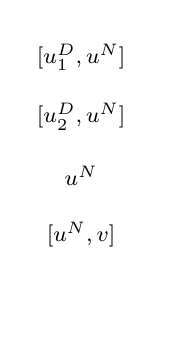
\begin{tikzpicture}
	    \begin{scope}[scale=0.75]
		\node at (0,0.5) {\footnotesize $\T{[u^N,v]}$};
		\node at (0,1.5) {\footnotesize $\R{u^N}$};
		\node at (0,2.5) {\footnotesize $\T{[u_2^D, u^N]}$};
		\node at (0,3.5) {\footnotesize $\T{[u_1^D, u^N]}$};
		\draw[white] (0,4)--(1,4);
		\draw[white] (0,-0.8)--(1,-0.8);
	    \end{scope}
	\end{tikzpicture}
    \end{subfigure}
    \begin{subfigure}{0.25\textwidth}
	\centering
	\begin{tikzpicture}
	    \begin{scope}[scale=0.75]
		\draw[thick] (0,0) -- (5,0);
		\draw[thick] (0,1) -- (5,1);
		\draw[thick] (0,2) -- (5,2);
		\draw[thick] (0,3) -- (5,3);
		\draw[thick] (0,4) -- (5,4);

		\draw[pattern=north east lines] (0.5,3) rectangle ++(2,0.7);
		\draw[fill=black!20] (1,3) rectangle ++(1.3,0.6) node[pos=.5] {$f_1$};
		\draw[<-, thick] (0.5,3.9) -- (0.5,3);

		\draw[pattern=north west lines] (1,2) rectangle ++(2,0.7);
		\draw[fill=black!20] (1,2) rectangle ++(1.8,0.6) node[pos=.5] {$f_2$};
		\draw[<-, thick] (1,2.9) -- (1,2);

		\draw[pattern=north east lines] (1.5,1) rectangle ++(1,0.7);
		\draw[pattern=north west lines] (2,1) rectangle ++(1,0.7);

		\draw[pattern=north west lines] (2.5,0) rectangle ++(2,0.7);
		\draw[pattern=north east lines] (2.5,0) rectangle ++(2,0.7);
		\draw[fill=black!20] (2.5,0) rectangle ++(1,0.6) node[pos=.5] {$f_2$};
		\draw[fill=black!20] (3.2,0) rectangle ++(1,0.6) node[pos=.5] {$f_1$};
	    \end{scope}
	\end{tikzpicture}
      \caption{Basic Consistency} \label{fig:exec_seq:basic_consistency}
    \end{subfigure}
    \begin{subfigure}{0.25\textwidth}
	\centering
	\begin{tikzpicture}
	    \begin{scope}[scale=0.75]
		\draw[thick] (0,0) -- (5,0);
		\draw[thick] (0,1) -- (5,1);
		\draw[thick] (0,2) -- (5,2);
		\draw[thick] (0,3) -- (5,3);
		\draw[thick] (0,4) -- (5,4);

		\draw[pattern=north east lines] (0.5,3) rectangle ++(2,0.7);
		\draw[fill=black!20] (0.5,3) rectangle ++(1.3,0.6) node[pos=.5] {$f_1$};
		\draw[<-, thick] (0.5,3.9) -- (0.5,3);

		\draw[pattern=north west lines] (1,2) rectangle ++(2,0.7);
		\draw[fill=black!20] (1,2) rectangle ++(1.8,0.6) node[pos=.5] {$f_2$};
		\draw[<-, thick] (1,2.9) -- (1,2);

		\draw[pattern=north east lines] (1.5,1) rectangle ++(1,0.7);
		\draw[pattern=north west lines] (2,1) rectangle ++(1,0.7);

		\draw[pattern=north west lines] (2.5,0) rectangle ++(2,0.7);
		\draw[pattern=north east lines] (2.5,0) rectangle ++(2,0.7);
		\draw[fill=black!20] (2,0) rectangle ++(1,0.6) node[pos=.5] {$f_1$};
		\draw[fill=black!20] (3.5,0) rectangle ++(1,0.6) node[pos=.5] {$f_2$};
	    \end{scope}
	\end{tikzpicture}
	\caption{GCL Consistency} \label{fig:exec_seq:gcl_consistency}
    \end{subfigure}
    \begin{subfigure}{0.25\textwidth}
	\centering
	\begin{tikzpicture}
	    \begin{scope}[scale=0.75]
		\draw[thick] (0,0) -- (5,0);
		\draw[thick] (0,1) -- (5,1);
		\draw[thick] (0,2) -- (5,2);
		\draw[thick] (0,3) -- (5,3);
		\draw[thick] (0,4) -- (5,4);

		\draw[pattern=north east lines] (0.5,3) rectangle ++(2,0.7);
		\draw[fill=black!20] (0.5,3) rectangle ++(1.5,0.6) node[pos=.5] {$f_1$};
		\draw[<-, thick] (0.5,3.9) -- (0.5,3);

		\draw[pattern=north west lines] (1,2) rectangle ++(2,0.7);
		\draw[fill=black!20] (1,2) rectangle ++(2,0.6) node[pos=.5] {$f_2$};
		\draw[<-, thick] (1,2.9) -- (1,2);

		\err at (3,2);

		\draw[pattern=north east lines] (1.5,1) rectangle ++(1,0.7);
		\draw[pattern=north west lines] (2,1) rectangle ++(1,0.7);

		\draw[pattern=north west lines] (2.5,0) rectangle ++(2,0.7);
		\draw[pattern=north east lines] (2.5,0) rectangle ++(2,0.7);
		\draw[fill=black!20] (3,0) rectangle ++(1,0.6) node[pos=.5] {$f_2$};
	    \end{scope}
	\end{tikzpicture}
	\caption{Stream Policing} \label{fig:exec_seq:stream_policing}
    \end{subfigure}
    \caption{Invalid execution sequences violating Basic Consistency (a), GCL Consistency (b), or Stream Policing (c)}
    \label{fig:exec_seq}
\end{figure*}
